% SBS2013 Presentation
% Scott Hendrickson
% @DrSkippy27
% Gnip Inc 

\documentclass{beamer}
\setbeamertemplate{navigation symbols}{}

% THEMES
\usetheme{gnip}

\usepackage[group-separator={,}]{siunitx}
%\usepackage{fontspec}
\setbeamertemplate{footline}[text line]{
    \colorbox{white}{\parbox[22px]{\paperwidth} {\color{linecolour} {\line(1,0){500} \\ \hfill Gnip Inc.   @DrSkippy27}}}
}

\beamersetuncovermixins{\opaqueness<1>{25}}{\opaqueness<2->{15}}

\usepackage{minted}
\usepackage{tikz}

\begin{document}
\title{Social Media Cocktail}  
\author{Scott Hendrickson \\ Data Scientist, Gnip Inc.\\ @DrSkippy27}
\date{\today} 

% title

\begin{frame}
\titlepage
\end{frame}

% staging the question

%\begin{frame}
%\begin{center}
%{\Huge getting the right mix \\ [5pt] for data-driven \\ [15pt] social marketing}
%\end{center}
%\end{frame}

% we believe

\begin{frame}
\begin{center}
\Huge social data has unlimited value and near limitless application
\end{center}
\end{frame}

% we believe
%
%\begin{frame}
%\begin{center}
%\Huge the source of record \\ for all public social conversation
%\end{center}
%\end{frame}

%  Why

\begin{frame}
\begin{center}
{\Huge why mix \\ [5pt] social media \\ [15pt] data? }
\end{center}
\end{frame}

% audience and perspective

\begin{frame}
\begin{center}
{\Huge <one> \\ [5pt]  audience, perspective, \\  [15pt] coverage }
\end{center}
\end{frame}

% volumes

\begin{frame} \frametitle{Audience -- Volume}
\begin{table}
\begin{tabular}{l|r}
\hline
   {Publisher}   &   {Daily Activity}   \\ [1pt]
\hline 
    Twitter      &      400M   \\
    Tumblr      &        75M   \\
    Wordpress Posts &     615k   \\
    Wordpress Comments & 1.1M \\
    Disqus       &       1.3M  \\
    Engagement (likes, votes) & 2.4M  \\
\hline
\end{tabular}
\end{table}
\end{frame}

\begin{frame}\frametitle{Gnip}
\Large{
\begin{itemize}
\item 4,600 Tweets/second \\ [2pt]
\item 1/2M unique Tumblr users/hour \\  [2pt]
\item PowerTrack filtering on data and metadata, PowerTrack Replay, Historical\ldots \\  [15pt]
\end{itemize}
}
\begin{center}
% 40K/second
\Huge{\emph{3B+ activities/day}}
\end{center}
\end{frame}

% signal vs. noise

\begin{frame}
\begin{center}
\center{\Huge {signal or noise?}}
\end{center}
\end{frame}

% chelsea con-ed example

\begin{frame}
  \begin{center}
    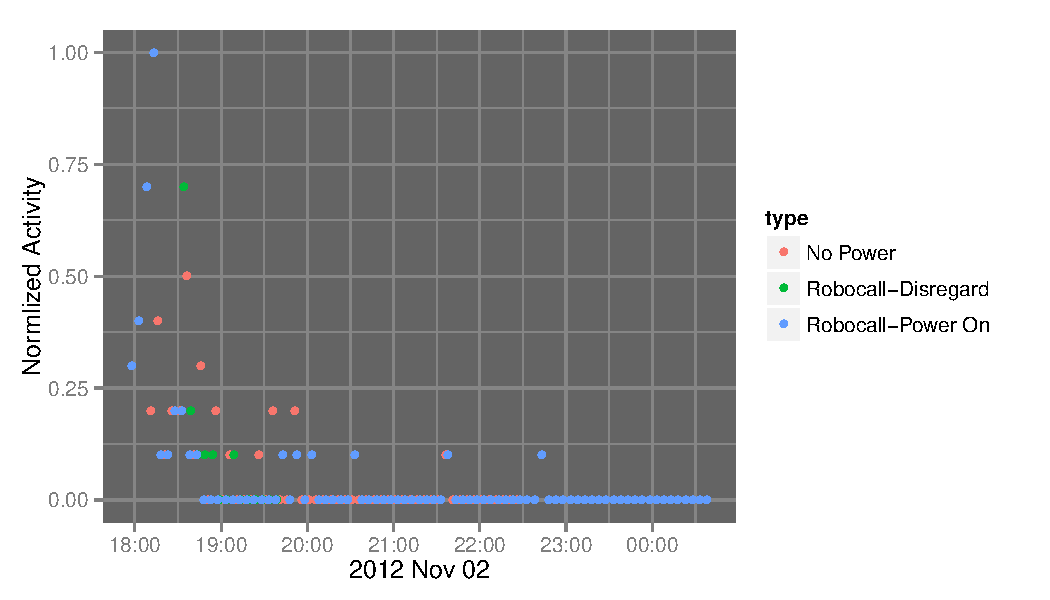
\includegraphics[width=8cm]{./imgs/fake.pdf}
  \end{center}
\end{frame}

\begin{frame}
  \begin{center}
    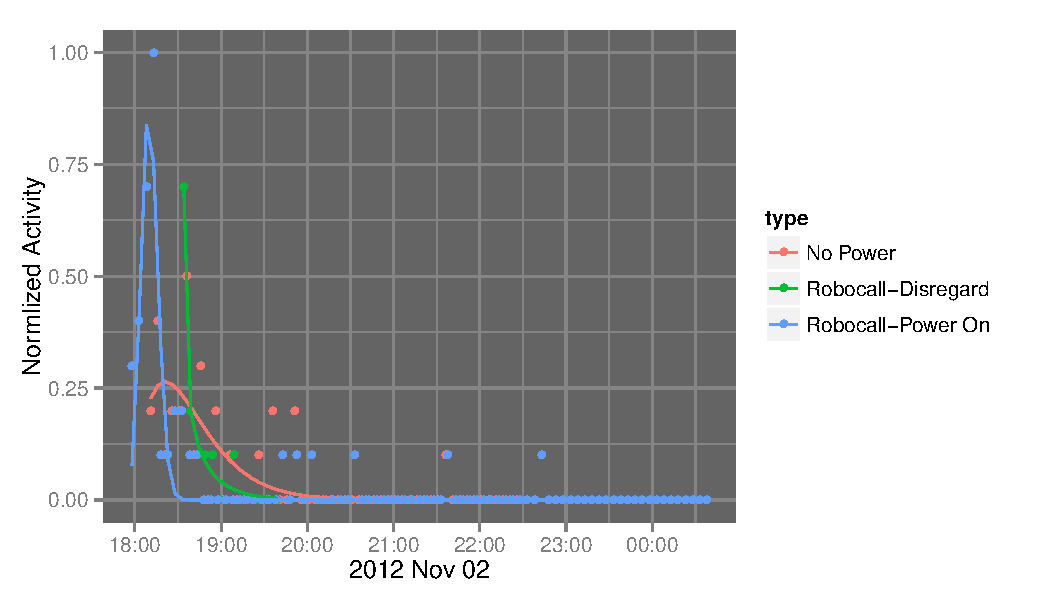
\includegraphics[width=8cm]{./imgs/fake_fit2.pdf}
  \end{center}
\end{frame}

%\begin{frame}
%  \begin{center}
%    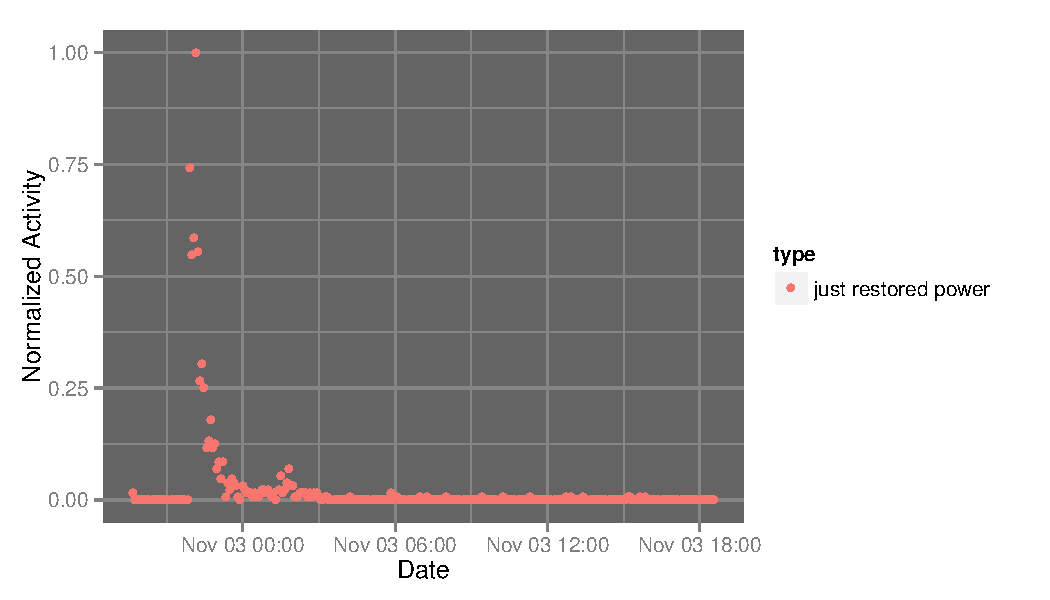
\includegraphics[width=8cm]{./imgs/real.pdf}
%  \end{center}
%\end{frame}

\begin{frame}
  \begin{center}
    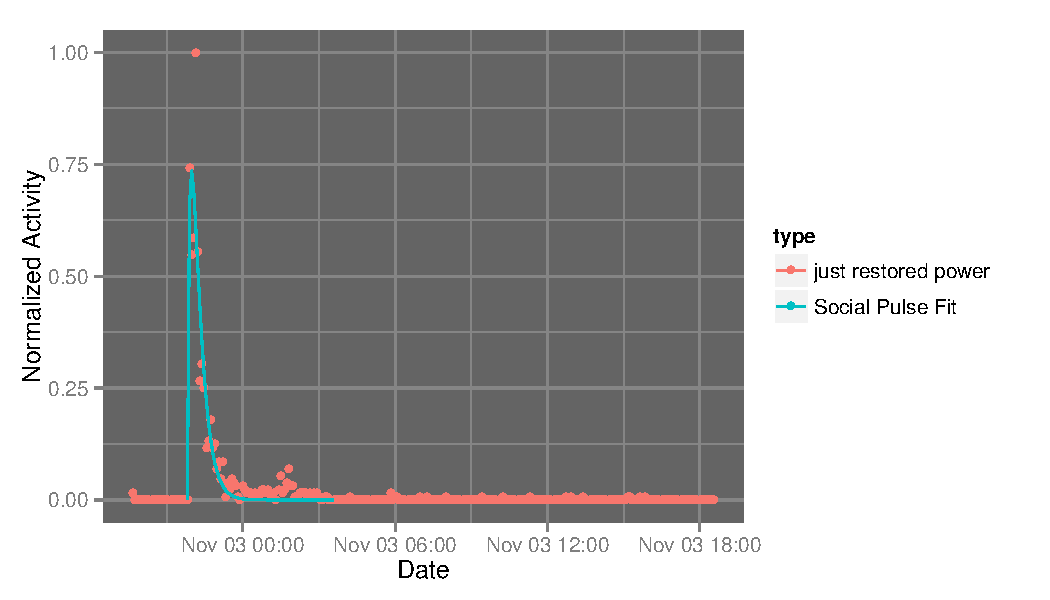
\includegraphics[width=8cm]{./imgs/real_fit.pdf}
  \end{center}
\end{frame}

% speed

\begin{frame}
\begin{center}
{\Huge <two> \\ [10pt] timing, evolution}
\end{center}
\end{frame}

% expected vs unexpected events

\begin{frame}\frametitle{Expected: Hurricane}
  \begin{center}
    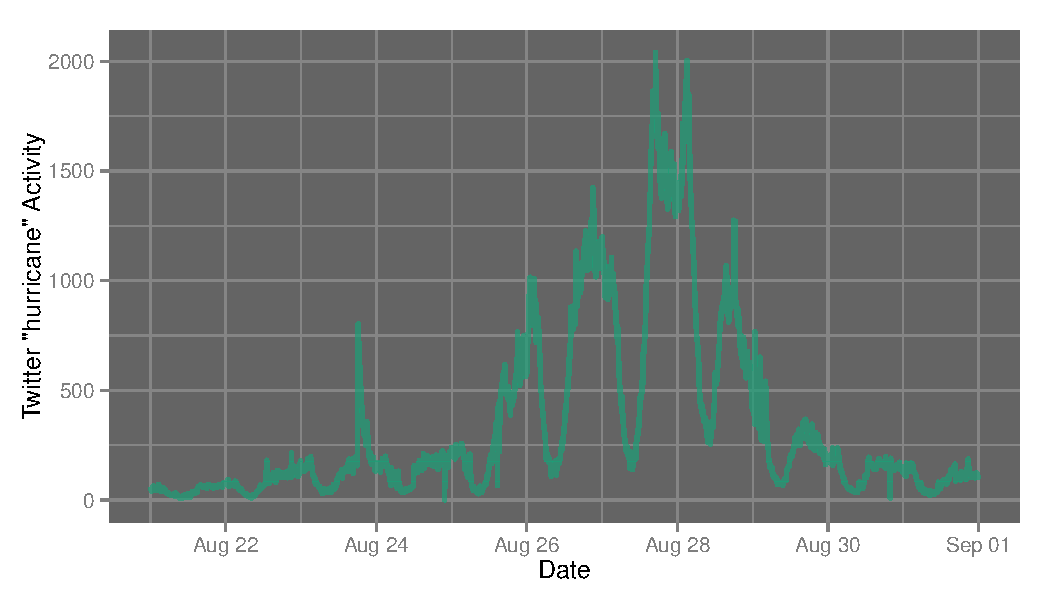
\includegraphics[width=8cm]{./imgs/hurricane.pdf}
  \end{center}
\end{frame}

\begin{frame}\frametitle{Expected: Hurricane}
  \begin{center}
    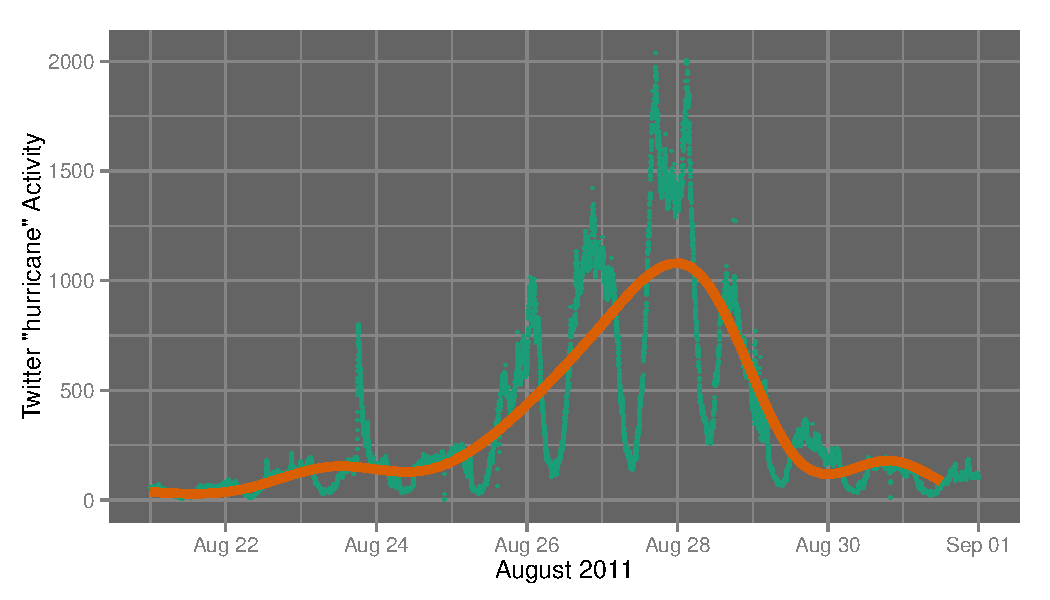
\includegraphics[width=8cm]{./imgs/hurricane_trend.pdf}
  \end{center}
\end{frame}

\begin{frame}\frametitle{Unexpected: Earthquake}
  \begin{center}
    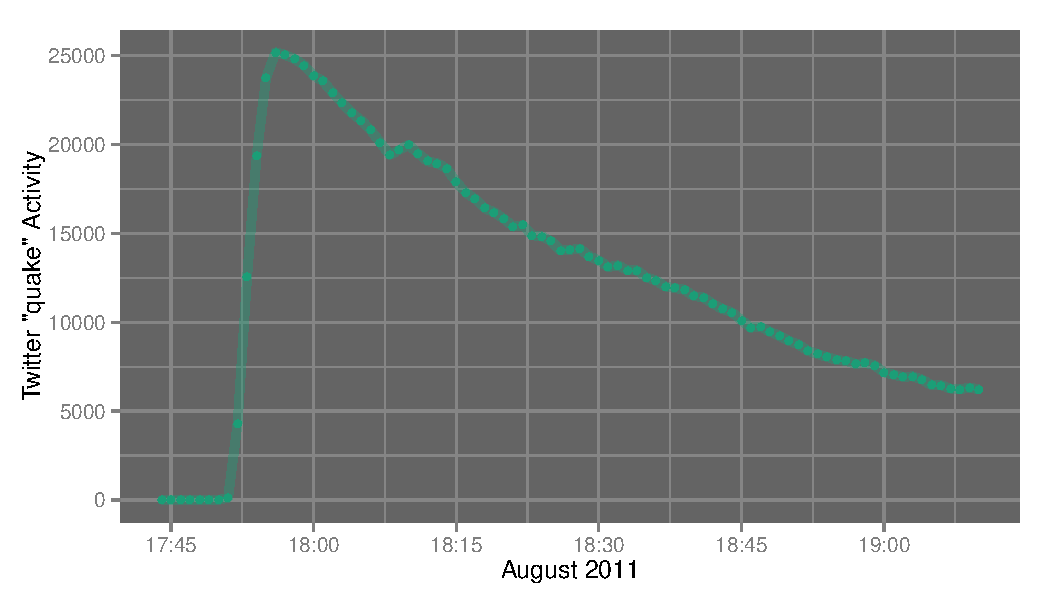
\includegraphics[width=8cm]{./imgs/va_quake.pdf}
  \end{center}
\end{frame}

\begin{frame}\frametitle{Unexpected: Earthquake}
  \begin{center}
    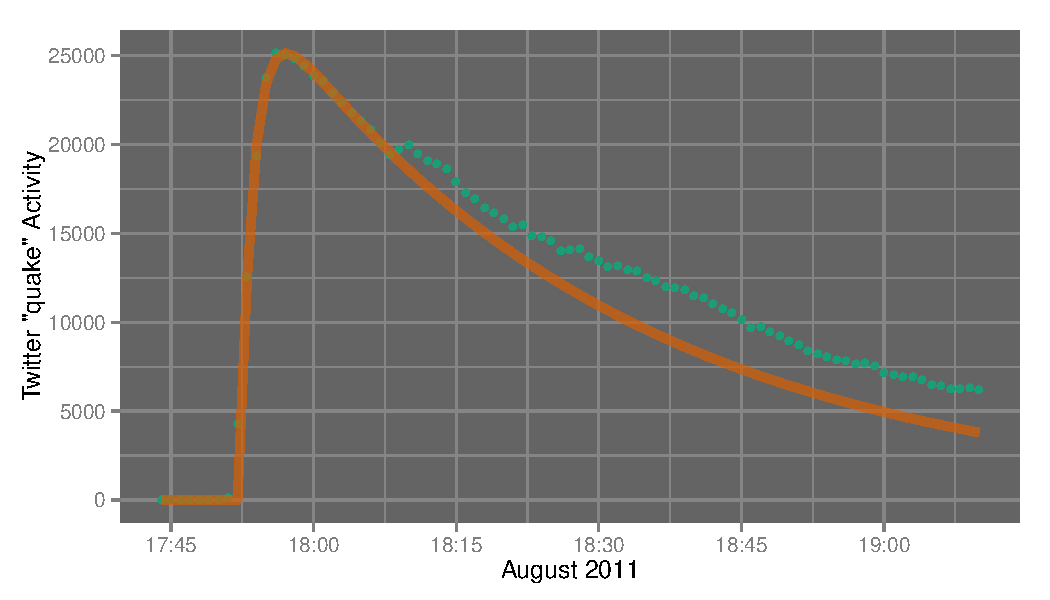
\includegraphics[width=8cm]{./imgs/va_quake_fit1.pdf}
  \end{center}
\end{frame}

% Events

\begin{frame}\frametitle{Classifying Events}
\begin{table}
\begin{tabular}{ m{2cm} | m{ 2.5cm} | m{4cm}}
\hline
Type & Response & Examples \\ \hline
Expected    & Approx. \newline Symmetric & Hurricane Sandy \newline Olympics \\ \hline
Unexpected (many obs.) & Social Media \newline Pulse & Beyonce' VMAs \newline  Mexico earthquake \newline  Steve Jobs \\ \hline
Unexpected (spread) & Network \newline Models & Osama Bin Laden \newline  Whitney Houston \newline  Syrian dissidents \\ \hline
\end{tabular}
\end{table}
\end{frame}

% half life

\begin{frame}\frametitle{Social Media Pulse Half-life}
\begin{center}
{\Huge time to observe \\[10pt] half of the activities}
\end{center}
\end{frame}

\begin{frame}
\frametitle{Social media pulse} 
Probability of an activity from one person,

\begin{equation*}
f(t) = \lambda \exp(-\lambda t), \text{ for } t \geq 0.
\end{equation*}

Many people, so sum random variables $S = X_1 + \ldots + X_{n}$.

Probability distribution function,

\begin{equation*}
f_S(t) = \frac{ \beta^{-\alpha} t^{\alpha-1} \exp( \frac{-t}{\beta}) } {\Gamma(\alpha)}
\end{equation*}

%Cumulative distribution is the ``generalized regularized incomplete gamma function'',
%
%\begin{equation*}
%F_S(t) = Q(\alpha, 0, \frac{ t}{\beta})
%\end{equation*}
\end{frame}

% gamma plots
%\begin{frame}
%  \begin{center}
%   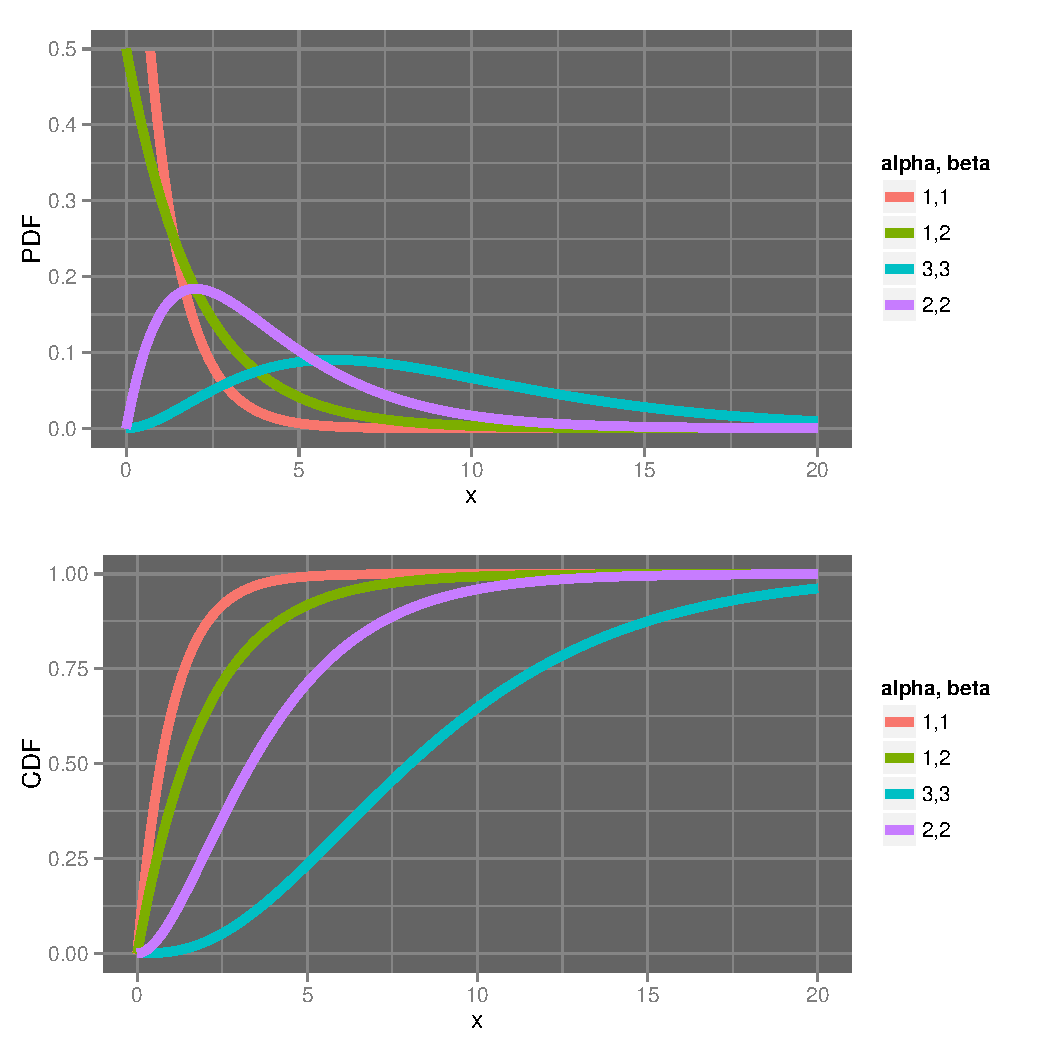
\includegraphics[height=6cm]{./imgs/gammadist.pdf}
%  \end{center}
%\end{frame}


\begin{frame}\frametitle{Why model half-life?}
\begin{center}
\begin{itemize}
\Huge{
\item predict total story volume
\item compare half-lives
\item anomalous story evolution
}
\end{itemize}
\end{center}
\end{frame}


\begin{frame}
  \begin{center}
    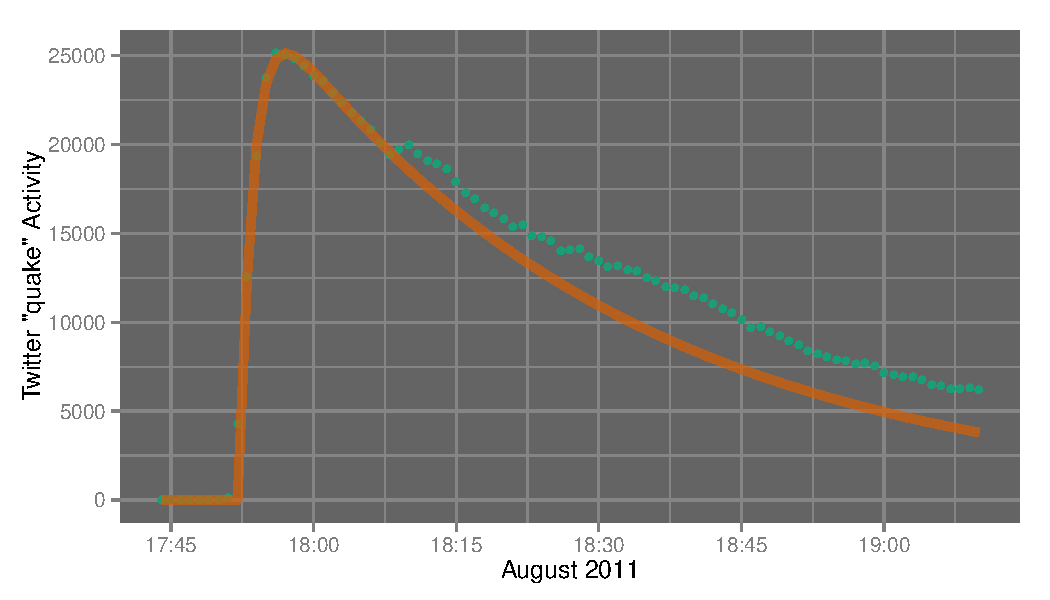
\includegraphics[width=8cm]{./imgs/va_quake_fit1.pdf}
  \end{center}
\end{frame}



\begin{frame} \frametitle{Story Timing}
\begin{table}
\begin{tabular}{l|c}
\hline
   {Publisher}   &   {Speed} \\
\hline 
    Twitter      &    Fast  \\ 
    Tumblr      &        Fast and Slow \\
    Wordpress Posts &   Fast and Medium   \\
    Wordpress Comments & Fast\\
    Disqus       &    Fast\\
    Engagement (likes, votes) &  Fast\\
\hline
\end{tabular}
\end{table}
\end{frame}

% JPMorgan

\begin{frame}
  \begin{center}
    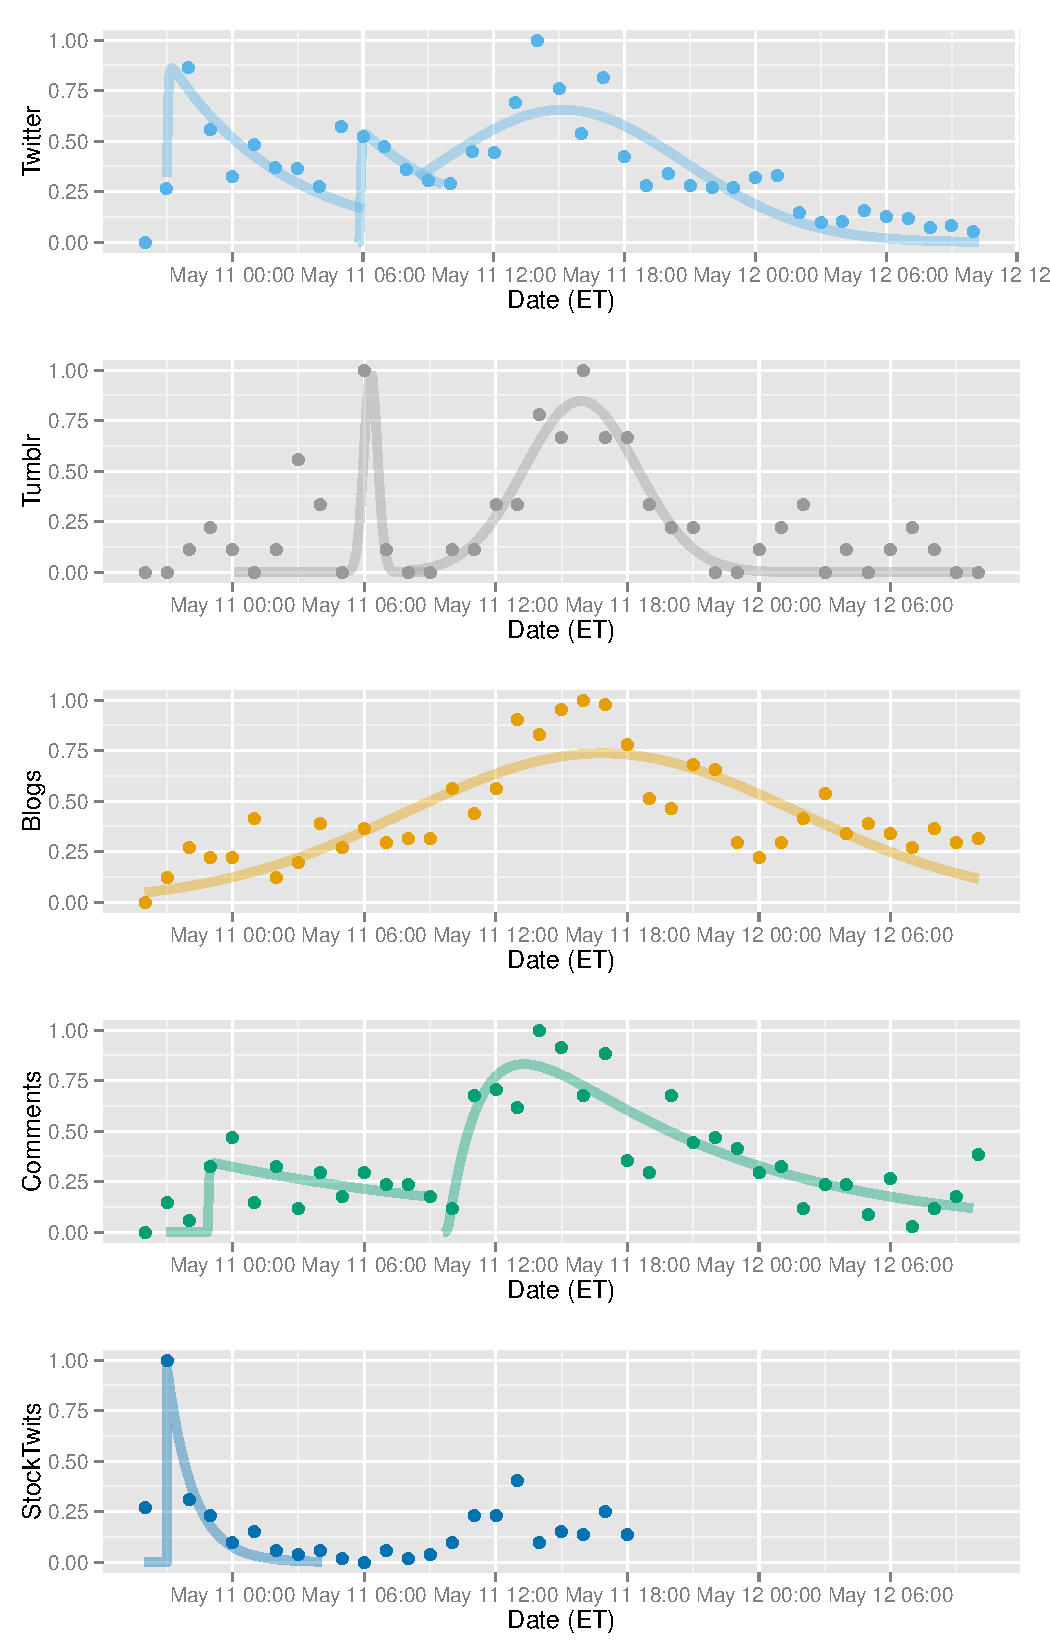
\includegraphics[height=8.5cm]{./imgs/JPMorgan.pdf}
  \end{center}
\end{frame}

%%  richness

\begin{frame}
\begin{center}
{\Huge <three> \\ [10pt] content richness }
\end{center}
\end{frame}


\begin{frame} \frametitle{Speed and Richness}
\begin{table}
\begin{tabular}{m{2cm}| c |m{3cm}}
\hline
   {Publisher}   &   {Speed} & {Richness} \\
\hline 
    Twitter       & Fast & Concise  \\ [3pt]
    Tumblr       & Fast, Slow & Rich, multimedia\\  [3pt]
    Wordpress Posts & Fast, Medium &  Rich, text\\  [3pt]
    Wordpress Comments  & Fast & Reactive, small-to-medium\\  [3pt]
    Disqus         & Fast & Reactive, small-to-medium\\  [3pt]
    Engagement   & Fast & Terse\\ 
\hline
\end{tabular}
\end{table}
\end{frame}

% summary speed and richness

\begin{frame}\frametitle{Social Cocktail}
  \begin{center}
    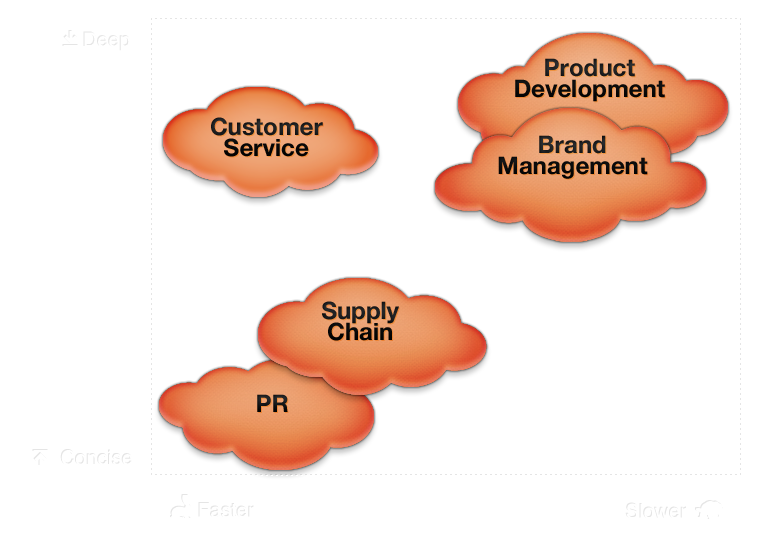
\includegraphics[width=7cm]{./imgs/socialcocktailgrid.png}
  \end{center}
\end{frame}



\begin{frame}
  \begin{center}
  \Large{Thank you!  \\ [20pt]}
    
\includegraphics[width=3cm]{./imgs/logo.png} \\ [15pt]
   \Large{Presentation, data, code at: github.com/DrSkippy27/SBS2013 }
  \end{center}
\end{frame}

\end{document}
